\documentclass[11pt]{article}
\usepackage[utf8]{inputenc}
% \usepackage[english, russian]{babel}
\usepackage[colorlinks=true,urlcolor=darkgray,citecolor=darkgray,linkcolor=darkgray,bookmarks=true]{hyperref}
% \usepackage{ccaption}
\usepackage{authblk}
\usepackage{indentfirst}
% \usepackage{float} 
\usepackage{amsmath}
% \usepackage{apacite}
\usepackage{natbib}
\usepackage{graphicx}
\usepackage{comment}
\usepackage{amsfonts}
\usepackage{bm}
\usepackage{amssymb}
\usepackage{amsthm}
\usepackage{mathtools}
\usepackage{upgreek} % AMS
\usepackage{marvosym}
\usepackage{threeparttable}
\usepackage{etoolbox}
\usepackage{cmap}	
\usepackage[nospace]{varioref}	
\usepackage{cleveref}
\usepackage{multirow}
\usepackage{fullpage} 
\usepackage{geometry}
\geometry{
 a4paper,
 total={210mm,297mm},
 left=20mm,
 right=20mm,
 top=20mm,
 bottom=20mm,
 }
\usepackage{url}
\usepackage{pgfplots}
\usepackage{caption}
\usepackage{longtable}
\usepackage{multirow}
\usepackage{booktabs}
\usepackage{pgf}
\usepackage{tikz}
\pgfplotsset{compat=1.15}
\usepackage{mathrsfs}
\usepackage{tikz} 
\usepackage{pgfplots}
\usepackage{pgfplotstable}
\usepackage{braket}
% \usepackage[capposition=top]{floatrow}
\usepackage{verbatim}
% \usepackage[position=bottom]{subfig}
\usepackage{graphicx}
%\usefonttheme[onlymath]{serif}
\usepackage[colorinlistoftodos]{todonotes}
\usepackage{setspace}
\usetikzlibrary{arrows}
\usetikzlibrary{calc}
\usetikzlibrary{positioning}
\usetikzlibrary{fit}
\usetikzlibrary{backgrounds}
\usetikzlibrary{intersections}
\tikzset{
style1/.style={
line cap=round,line join=round,
axis/.style={thick, ->, >=stealth'},
l/.style={thin},
d/.style={dashed, thin}, 
pile/.style={thin, <->, >=stealth',shorten <=3pt, shorten >=3pt}, 
every node/.style={color=black}, 
}
}




% \usepackage[backend=biber,
% style=chicago-authordate]{biblatex}
% \addbibresource{references.bib}

\def\references{
    \bibliography{misc/references.bib}
    \bibliographystyle{misc/econ}
}



\usepackage{parskip}

\setlength{\parindent}{15pt}
\onehalfspacing

    \makeatletter 

% \renewcommand{\maketitle}{\begin{center}
%         \noindent{\bfseries\scshape\Large\@title} 
%         \noindent{ \itshape\large\card{\subtitle}} 
%         \par  \vspace{0.5ex}
%         \noindent {\large\itshape\@author}
%         \noindent{\card{\footnotesize \itshape \extratext}}
%         \end{center}
%         } 

    % \makeatother
    % \def\extratext{}
    % \def\topic{}
    % \def\subtitle{}
       
 \newcommand{\card}[1]{ \ifthenelse{\equal{#1}{}}{}{ {\par#1}}}

 \usepackage{lipsum}

 \makeatletter
 \def\blfootnote{\gdef\@thefnmark{$\dagger$}\@footnotetext}
 \makeatother




    %%% Работа с картинками
    \usepackage{graphicx}  % Для вставки рисунков
    \setlength\fboxsep{3pt} % Отступ рамки \fbox{} от рисунка
    \setlength\fboxrule{1pt} % Толщина линий рамки \fbox{}
    \usepackage{wrapfig} % Обтекание рисунков текстом
    \usepackage{rotating}%поворот figure


    \DeclareRobustCommand{\firstsecond}[2]{#1}


    \makeatletter
\newcommand\footnoteref[1]{\protected@xdef\@thefnmark{\ref{#1}}\@footnotemark}
\makeatother


\usepackage{rotating}
% \usepackage{caption}
\usepackage{subcaption}
\captionsetup{labelfont=bf, labelsep=period, skip=0pt}


\graphicspath{{./../Figures}}


\usepackage{makecell}
\usepackage{dcolumn}

\title{State-Dependent Systematic Monetary Policy}
\author{Alexander I. Vlasov\thanks{Email: avlasov(at)nes.ru. For supplementary materials, code and datasets, see the repository \href{https://github.com/alvlsv/CheckingHank}{github.com/alvlsv/CheckingHank}. I thank Valery Charnavoki and Konstantin Styrin for helpful comments.}}
\date{\normalsize First version: January, 2024\\\vspace{1ex} This version: May, 2024\\ \vspace{1ex}
\href{https://github.com/alvlsv/CheckingHank/blob/6906f23fcb1a16aa4fc9997532f52c1659e9c29f/Checking_HANK/Paper/CheckingHANK.pdf}{Click here for the most recent draft}}


\begin{document}

% \maketitlenew
% \selectlanguage{english}
\maketitle



\begin{abstract}
    \noindent This work estimates the time-varying Taylor Rule the systematic monetary policy. 
    \\
    \noindent\textbf{Keywords:} Monetary Policy
    \\
    \noindent\textbf{JEL Codes:} E21, E52, E12 \\
    \bigskip
\end{abstract}

\section{Introduction}

% The prerequisite for the successful conduction of monetary response to a shock is the good understanding of Monetary Transmission Mechanism (MTM) -- the way that external changes in short term rate translate into the economy. 
% Traditionally, macroeconomic models assumed away all of the heterogeneity in agents, replacing each with a representative one \cite{Gali2018}.
% This representative agent models are distinguished by the fact that they show the economy in a much more compact and tractable manner than heterogeneous ones.
% Although, assumption of insignificance of differences between households looks quite unrealistic, it is still not immediately obvious, whether heterogeneity in a particular agent traits actually enhances the predictive powers of Representative-Agent New Keynesian (RANK) models\footnote{For example, \citet{Krusell1998} argue that  ``the behavior of the macroeconomic aggregates can be almost perfectly described using only the mean of the wealth distribution''.} 
% and whether this result would hold to the data.

% This paper conduct an econometric check of one of distinct outcomes of Heterogeneous-Agent New Keynesian (HANK) model by \citet[henceforth, KMV]{KMV2018}, namely size-persistence tradeoff. 


% One of the most important problem in RANK is that, in equilibrium all of the agents are neither savers nor borrowers, even in the absence of financial frictions \cite{Gali2018}. 
% This happens because every agent in the model is identical, and therefore, the only possible channel through which monetary policy could work, in theory, is the intertemporal substitution channel.
% But this this questioned by the fact that aggregated time-series data on consumption finds a small sensitivity of consumption to changes in the interest rate after controlling for income changes \cite{Campbell1989, Canzoneri2007} -- ``imperfect consumption insurance''. 
% Although by itself, it cannot be concluded from this evidence that the effect of intertemporal substitution is small, because indirect effects can almost completely compensate for changes caused by substitution.


% \citet{KMV2018} served as a way to answer the accumulated questions about modeling the economy in a neo-Keynesian manner. 
% The key idea is that some of the households face financial frictions i.e borrowing limit, which make them more sensitive to income change and less sensitive to shock of interest rate, since household cannot smooth the unexpected temporal income shock with the increase in credit.


% \subsection{Trade-offs in HANK}

% HANK, since it was not reversely-engineered, requires not only a ``check for inputs''\footnote{The Hand-to-Mouth household existence, which was done in  \citet{KVW2014}, and in \citet{Cloyne2019}.} but also a ``check for outputs'' -- the monetary policy outcomes.
% HANK, as formulated by KMV has two main monetary policy tradeoffs:
% tradeoff between size and persistence of monetary shock, and inflation-activity tradeoff.
% In this work we focus on the former tradeoff.
% It could be summarized as following: the higher the autocorrelation of monetary shock, the lower the elasticity of consumption to the expected path deviation of the rate of interest from its natural value.\footnote{Further we sometimes  refer to a difference between real rate and neutral (natural) rates of interest as the excess rate}
% Intuitively, persistence of highly autocorrelated shock is indifferent to non-HtMs, as it is in RANK, since the only channel of monetary transmission is intertemporal substitution, but it matters for HtM households, whose response may be dampened by the persistence of monetary shock. 
% This effect stems from failure of Ricaridan equivalence, since when it fails, then ``not only timing of fiscal policy but timing of monetary policy matters as well'' \cite{KMV2018}.

The conduct of monetary policy can be divided via two axis (see \vref{tab:taxonomy}), the systematicality of a policy and the expectations of the market from the actions of monetary authority. 
The examples of monetary policy cells along the main diagonal of \vref{tab:taxonomy} are the most frequent uses of systematic and unsystematic monetary policies, but note that the off diagonal elements are not empty.

\begin{table}[h!]\centering 
  \begin{threeparttable}
  \caption{Monetary Policy Taxonomy}
  \label{tab:taxonomy}
  \begin{tabular}{@{\extracolsep{5pt}}lcc} 
    \\[-1.8ex]\hline 
    \hline \\[-1.8ex] 
    & Systematic & Unsystematic\\ 
    \hline \\[-1.8ex] 
    Anticipated& \makecell[c]{Known monetary \\ policy function} & \makecell[c]{Credible announcement\\ of a transitory policy}\\ \\
    Unanticipated & \makecell[c]{Changes to \\ monetary policy function} & Monetary shocks\\
    \\[-1.8ex]\hline 
    \hline
  \end{tabular}
  \begin{tablenotes}[flushleft]\footnotesize
    \item[]\textit{Notes:} Idea of the distinction is from \citet{JordaHoover2000}, who use it with regards to central bank's policy of money supply.
  \end{tablenotes}
\end{threeparttable}
\end{table}


\subsection{Related literature}

\citet{Carvalho2021} argues for estimation of Taylor rule using the OLS because the monetary policy shocks tend to explain only a small fraction of the overall variation of monetary instruments (i.e. Fed Funds rate, FFR).

% First, this work provides additional indirect empirical support for models focused on the role of heterogeneity in household portfolio in MTM, for example \citet{KMV2018}, \citet{Auclert2019}, \citet{Luetticke2021} and successors.
% There were several studies, which empirically support HANK. 

% Most of the literature exploring the empirical side of HANK uses the individual level portfolio data. \citet{HolmPaulTischbirek2020} explores the norwegian individual-level dataset in trying to investigate the full process of the transmission of monetary policy.
% They find that the low-liquidity households (\citeauthor{KMV2018} would call them hand-to-mouth households) show strong response to monetary shock estimated with \cite{RomerRomer2004} identification strategy.
% Another work lying in the same field is \citet{Cloyne2019}, which  shows that aggregate response of consumption to interest rate is mostly driven by households with a mortgage -- balance sheet driven heterogeneity plays a key role in monetary policy transmission.
% It finds, that, in response to a negative monetary shock, the expenditure rise is highly significant for mortgagors\footnote{As \citet{Cloyne2019} shows, mortgagors and Wealthy HtMs as defined by \citet{KVW2014} are extremely overlapping groups.}, less significant for renters, and insignificant for owners with controls for different characteristics.
% Another empirical contribution to of literature is done by \citet{Gross2020}, they document the MPC change over economic cycle, specifically its change through GFC.

%add
This work contribute to. Additionally we this work is one of the first, that uses newly developed way of identification of systematic monetary policy  by , which allows us to estimate the aforementioned overall effect of the monetary shock, without controlling for any income related covariates -- without possible .


The remainder of the paper proceeds as follows: 
the next section thoroughly discloses the empirical strategy for estimating time-varying (or FOMC preference dependent) Taylor rule.
Than I describe and the results and conclude.



\section{Empirical Strategy}
\subsection{Systematic Monetary Policy Identification}

Further I follow \citet{HIM2023} approach to systematic monetary policy identification that is based on the use of Hawk-Dove balance as a measure of systematic monetary policy variation. That is, I assume that the monetary policy rule is 
\begin{equation}
  r_t-r_t^*=\tilde\phi_{t}^\pi \mathbb{E}_t\pi_{t+1} +\tilde\phi_{t}^x \mathbb{E}_tx_{t}+\varepsilon_t,\label{eq:Taylor1}
\end{equation}
where $r_t$ is the real rate of interest, $r_t^*$ is the natural rate of interest $\pi_{t+1}^e$ and $x_{t+1}^2$ are the monetary authority's expectations over the inflation and output gap. As one can see Then $\tilde \phi_t^{j}=\phi^j+\phi_t^j$ is the systematic monetary policy -- that is, the time-dependent response of the monetary authority to the expected change in inflation/output. 

The assumed monetary policy rule is essentially a Taylor rule, but also it can be viewed as a simplified time-varying version of \citet{RomerRomer2004} regression rule.

I estimate the following state-dependent local projection model 
\begin{multline}
    r_{t+h}-r^*_{t+h}=\alpha^h+\delta^h\left(\mathit{Hawk}_{t}-\overline{\mathit{Hawk}}\right)\\ +\beta_\pi^h \pi_{t}^e+\gamma_\pi^h \pi_{t}^e\left(\mathit{Hawk}_{t}-\overline{\mathit{Hawk}}\right)+\beta_x^h x_{t}^e+\gamma_x^h x_{t}^e\left(\mathit{Hawk}_{t}-\overline{\mathit{Hawk}}\right)\\+\zeta^hZ_t+e_{t+h}^h,\label{eq:LP1}
\end{multline}
where $h=0,\dots, H$ are the forecast horizons. $r_{t+h}$ is federal funds rate (bridged with \citet{WuXia2016} for the ZLB period) and $r^*_{t+h}$ is the \citet{LW2003} natural interest rate.\footnote{I use \citet{HLW2023} updated version of the \citet{LW2003} natural rate.}
$\pi_t^e$ is the measure of the FED expectation of future inflation. I use the average of the one- and two-quarters  tealbook inflation forecast following the approach by \citet{CoibionGorodnichenko2011}. 
$\mathit{Hawk}_t$ is the quarterly Hawk-Dove index of \citet{HIM2023}, which is based on the \citet{Istrefi2019} and \citet{BordoIstrefi2023} estimation of individual policy preference of FOMC members expressed before each of the FOMC meeting in press; $\overline{\mathit{Hawk}}$ stand for the mean of this variable. 

The vector of controls, $Z_t$, consists of the 4 lags of the dependent variable, $\left(r-r^*\right)_t$, 4 lags of the expected inflation, $\pi_t^e$, and 4 lags of expected gdp gap, $x_t$.

As \citet{HIM2023} suggest, the Hawk index, $\mathit{Hawk}_t$, can be potentially endogenous,\footnote{The FOMC member's preferences, although persistent, can reflect the changes in economic environment or preference of a president who appoints new members, which also may depend on the business cycle state.}
The proposed solution is to instrument $\left(\mathit{Hawk}_{t}-\overline{\mathit{Hawk}}\right)$ with the index of preferences of the rotating part of FOMC board\footnote{Since 1940 each year 4/12 FOMC memberships rotate among 11 FRB presidents. Cleveland and Chicago get a seat every second year and Philadelphia, Richmond, Boston, Dallas, Atlanta, St. Louis, Minneapolis, San Francisco, Kansas City -- every third year. By construction this rotation is independent of the business cycle.} namely $\left(\mathit{Hawk}_{t}^\mathit{IV}-\overline{\mathit{Hawk}}^\mathit{IV}\right)$.

The instrument vector in this case is 
\[\begin{bmatrix}
  1& \pi_t^e& x_t^e& \pi_t^e\times\left(\mathit{Hawk}_{t}^\mathit{IV}-\overline{\mathit{Hawk}}^\mathit{IV}\right)& x_t^e\times\left(\mathit{Hawk}_{t}^\mathit{IV}-\overline{\mathit{Hawk}}^\mathit{IV}\right)
\end{bmatrix}\]

Note that the contemporaneous tealbook estimates of the GDP gap and CPI inflation are available only starting from 1987:Q3 and 1979:Q4, respectively. 
Also all Tealbook series are restricted 2018 Q4 due to 5 year publication lag, what leaves only 124 observations. 
In order to increase the time-span of the Taylor rule estimated in \vref{eq:LP1}, I replace the projected CPI inflation with projected deflator inflation and projected GDP gap with projected unemployment gap.\footnote{I define projected unemployment gap as the difference between tealbook projection of unemployment and projection of NAIRU. As previously, following \citet{CoibionGorodnichenko2011}, the projection is an average between T+1 and T+2 projections.} Under the replaced measures of inflation and output gap (as unemployment gap) the sample size grows to 202 observations, starting from 1968:Q1.

So, I end up estimating 2 specifications: the specification with projected CPI inflation and projected GDP gap, which I name \emph{short specification}, and the specification with projected GDP price inflation and unemployment gap, named \emph{long specification}. 
Both specifications, assuming stable Okun's law (linear relation between GDP gap and unemployment gap), essentially measure the same Taylor rule, but using different measures for inflation and gap in economic activity. 


\subsection{Endogeneity Bias}

Note, that ideally in order to estimate \vref{eq:LP1} we want to instrument not only $\mathit{Hawk}_{t}$ but also the other main variables of interest, namely FOMC inflation and output gap projections. 
In order to find some orthogonal variation

\citet{Carvalho2021} argues that the monetary policy shocks tend to explain a small fraction\footnote{Also note that due to the increasing use of policies that rely on expectations management (i.e. forward guidance), central banks have become more opened, what leads to decrease in share of movement in rates due to monetary policy shocks.} of the variance of regressors typically included in monetary policy rules, the endogeneity bias tends to be small.

\section{Results}

\subsection{Response to expected Inflation and Output gap}

\subsubsection{Short Specification}
The estimated coefficients of interest of the short regression can be found in \vref{fig:LP_short,tab:LP_short}. 
They are mean and differential response to a unit increase in tealbook projected CPI inflation and GDP gap. 
The differential responses is shown under the deviation of $\mathit{Hawk}_t$ from its mean equal to $2/12$, which is slightly higher than one standard deviation. The coefficients for several selected quarters for the main regressors of interest can be seen in \vref{tab:LP_short}. 

The average response of the $(r-r^*)$ are larger than zero up on 95\% confidence to 8th quarter. 
The impact of hawkishness of FOMC on the effect of a change in projected inflation becomes prominent after 3rd quarter and is negative, that is the additional 2 hawk members of FOMC reduce the response to inflation by 0.3 percentage points starting from the 3rd quarter. Note that the effect of hawks on response to inflation becomes not distinguishable from zero from the 7th quarter.




\begin{figure}[!htbp]\centering
  \begin{minipage}{0.9\textwidth}
    \caption{Policy Response to Inflation and FOMC Hawkishness. Short Specification}\vspace{2ex}
    \label{fig:LP_short}
    \begin{subfigure}[b]{0.495\textwidth}
        \centering
        \caption{Average Resp. to Projected CPI Inflation}
        \label{fig:LP_short:average_inflation}
        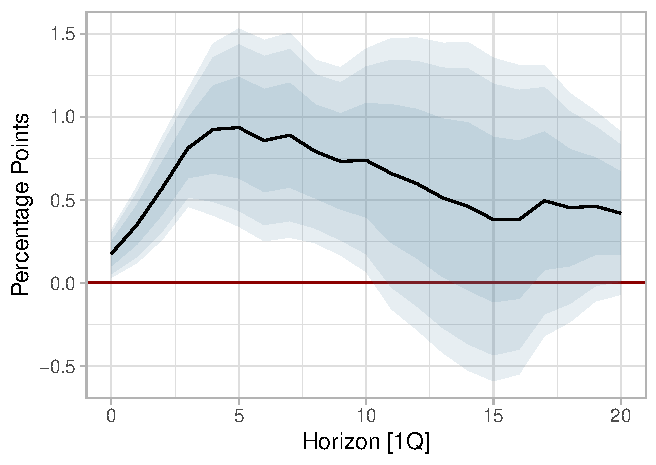
\includegraphics[width=\linewidth]{average_cpi_inflation_short.pdf}
    \end{subfigure}
    \hfill
    \begin{subfigure}[b]{0.495\textwidth}
        \centering
        \caption{Differential  Resp. to Projected CPI Inflation}
        \label{fig:LP_short:differential_inflation}
        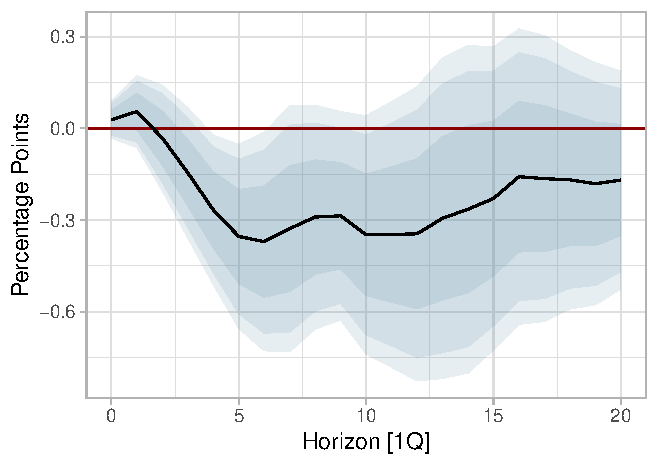
\includegraphics[width=\linewidth]{differential_cpi_inflation_short.pdf}
    \end{subfigure}\vspace{2ex}
    \begin{subfigure}[b]{0.495\textwidth}\centering
      \caption{Average Resp. to Projected GDP Gap}
      \label{fig:LP_short:average_gap}
      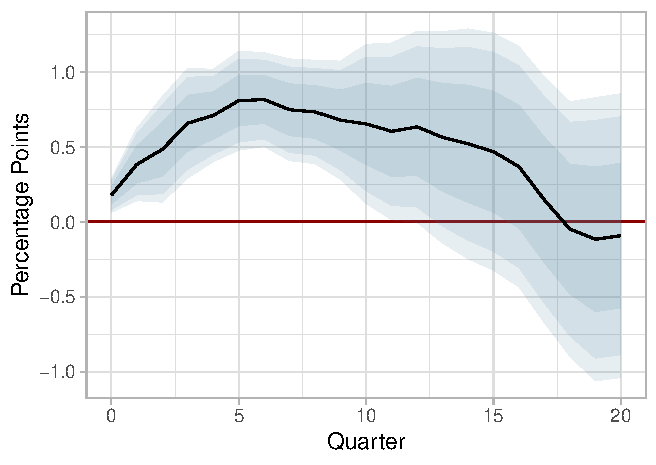
\includegraphics[width=\linewidth]{average_gap_short.pdf}
    \end{subfigure} \hfill
    \begin{subfigure}[b]{0.495\textwidth}\centering
      \caption{Differential Resp. to Projected GDP Gap}
      \label{fig:LP_short:differential_gap}
      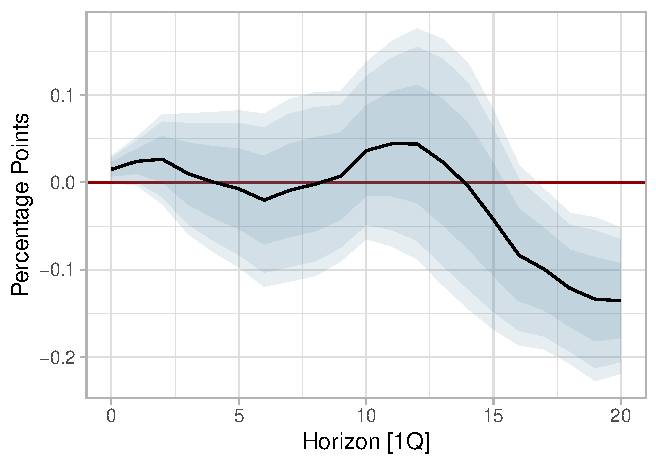
\includegraphics[width=\linewidth]{differential_gap_short.pdf}
    \end{subfigure}
        {\begin{flushleft}\scriptsize\textit{Notes}: This figure reports the responses of the $(r-r^*)_t$ to an increase in the Tealbook CPI inflation forecast and GDP gap forecast of 1 p.p. The subfigure \ref{fig:LP_short:average_inflation} reports the response of $(r-r^*)_t$ to projected CPI inflation for the $\mathit{HAWK}$ index equal to the sample average; \ref{fig:LP_short:differential_inflation} is the addition to the response in case there are 2 (out of 12 in total) additional consistent hawks in the FOMC. Subfigures \ref{fig:LP_short:average_gap} and \ref{fig:LP_short:differential_gap} report the same for the increase in projected GDP gap for 1p.p. The shaded areas correspond to 68\%, 90\% and 95\% confidence bands calculated with HAC estimator with \citet{Andrews1991} weighting.\end{flushleft}}
            
  \end{minipage}
\end{figure}




\begin{table}[!hbtp]\centering \footnotesize
  \begin{threeparttable}
    \caption{Estimates of Short LP Taylor Rule}
    \label{tab:LP_short}
    \begin{tabular}{@{\extracolsep{5pt}}lccccccc} 
      \\[-1.8ex]\hline 
      \hline \\[-1.8ex] 
       & \multicolumn{7}{c}{\textit{Dependent variable:} $\left(r-r^*\right)_{t+h}$} \\  
       \\[-1.8ex]
      \cline{2-8} 
      \\[-1.8ex] & $h=0$ & $h=2$ & $h=4$ & $h=6$ & $h=8$ & $h=10$ & $h=12$ \\ 
      \\[-1.8ex] & (1) & (2) & (3) & (4) & (5) & (6) & (7)\\ 
      \hline \\[-1.8ex] 
       Expected CPI Inflation, & 0.175$^{**}$ & 0.570$^{***}$ & 0.923$^{***}$ & 0.856$^{***}$ & 0.791$^{***}$ & 0.738$^{**}$ & 0.596 \\ 
        $\Delta\mathit{CPI}_t^e$ & (0.073) & (0.157) & (0.263) & (0.308) & (0.281) & (0.342) & (0.448) \\ 
       & & & & & & & \\ 
       $\quad \times \left(\mathit{Hawk}_t-\overline{\mathit{Hawk}}\right)$ & 0.170 & $-$0.191 & $-$1.600$^{**}$ & $-$2.224$^{**}$ & $-$1.741 & $-$2.091$^{*}$ & $-$2.070$^{*}$ \\ 
       & (0.186) & (0.530) & (0.749) & (1.094) & (1.122) & (1.193) & (1.193) \\ 
       & & & & & & & \\ 
       Expected GDP Gap, $x_t^e$ & 0.177$^{***}$ & 0.483$^{***}$ & 0.709$^{***}$ & 0.815$^{***}$ & 0.733$^{***}$ & 0.653$^{**}$ & 0.633$^{*}$ \\ 
       & (0.058) & (0.180) & (0.157) & (0.160) & (0.176) & (0.271) & (0.325) \\ 
       & & & & & & & \\ 
       $\quad \times \left(\mathit{Hawk}_t-\overline{\mathit{Hawk}}\right)$ & 0.089$^{*}$ & 0.158 & 0.002 & $-$0.122 & $-$0.013 & 0.217 & 0.263 \\ 
       & (0.046) & (0.156) & (0.244) & (0.302) & (0.320) & (0.308) & (0.308) \\ 
       & & & & & & & \\ 
       $\left(\mathit{Hawk}_t-\overline{\mathit{Hawk}}\right)$ & $-$0.146 & 0.875 & 3.991$^{*}$ & 6.539$^{**}$ & 7.241$^{**}$ & 8.725$^{**}$ & 7.998$^{**}$ \\ 
       & (0.446) & (1.321) & (2.151) & (3.167) & (3.432) & (3.640) & (3.928) \\ 
       & & & & & & & \\ 
       \hline \\[-1.8ex] 
       Observations & 122 & 122 & 122 & 122 & 122 & 120 & 118 \\ 
       R$^{2}$ & 0.983 & 0.912 & 0.784 & 0.647 & 0.528 & 0.416 & 0.373 \\ 
       Adjusted R$^{2}$ & 0.981 & 0.898 & 0.749 & 0.590 & 0.451 & 0.318 & 0.266 \\ 
       Residual Std. Error & 0.322 & 0.716 & 1.063 & 1.295 & 1.457 & 1.582 & 1.622 \\ 
       Wu-Hausman & 0.395& 0.352& 0.718& 1.891& $6.496^{***}$ &$15.97^{***}$& $15.05^{***}$ \\ \hline 
       \hline 
    \end{tabular}
    \begin{tablenotes}[flushleft]\scriptsize
      \item \textit{Notes:} 
      This table reports the estimates of the coefficients of interest in model in \vref{eq:LP1} with projected inflation measured as a projected change in CPI. 
      The \citet{Andrews1991} HAC standard errors are in parenthesis. 
      All of the coefficients can be seen in \vref{tab:LP_short_full}. 
      Weak Instrument F-statistics (for $h=0$) are HAWK: $53.5^{***}$; interaction with CPI inflation: $42.2^{***}$, interaction with GDP gap: $51.4^{***}$. $^{*}p<0.1$; $^{**}p<0.05$; $^{***}p<0.01$.
    \end{tablenotes}
    \end{threeparttable}  
    \end{table}
  
  



\subsubsection{Long Specification}

\citet{HIM2023} (in appendix named ``Validation Exercise'') estimates the model similar to \vref{eq:LP1} under long specification, but under assumption that the systematic monetary policy responds only to inflation. My estimates in \vref{fig:LP_long} and \vref{tab:LP_long} average and differential responses of $r_t-r_t^*$ to CPI inflation tend to be smaller compared to the estimations of \citet{HIM2023}. 
The difference is due to the fact that \citet{HIM2023} 1) do not correct the fed funds rate for the natural rate of interest, i.e. estimate the response of $r_t$, and 2) assume that the monetary authority systematic policy respond only to inflation. 




\begin{figure}[!htbp]\centering
  \begin{minipage}{0.9\textwidth}
  \caption{Policy Response to Projected Deflator Inflation and Unemployment Gap and FOMC Hawkishness. (Long Specification)}\vspace{2ex}
  \label{fig:LP_long}
  \begin{subfigure}[b]{0.495\textwidth}
      \centering
      \caption{Average Resp. to Deflator Inflation}
      \label{fig:LP_long:average_inflation}
      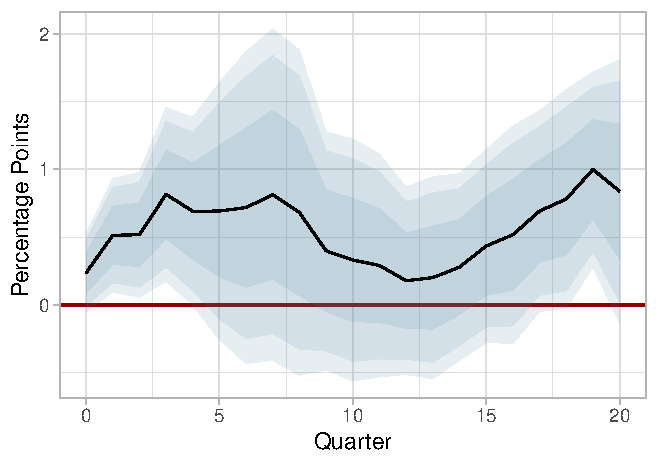
\includegraphics[width=\linewidth]{average_deflator_inflation_long.pdf}
  \end{subfigure}
  \hfill
  \begin{subfigure}[b]{0.495\textwidth}
      \centering
      \caption{Differential Resp. to Deflator Inflation}
      \label{fig:LP_long:differential_inflation}
      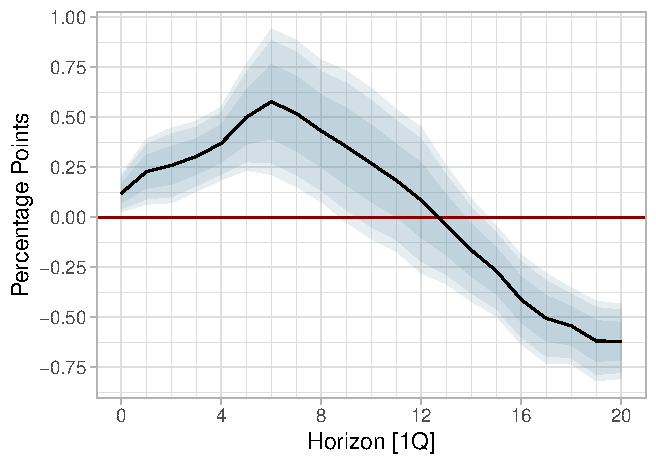
\includegraphics[width=\linewidth]{differential_deflator_inflation_long.pdf}
  \end{subfigure}\vspace{2ex}
  \begin{subfigure}[b]{0.49\textwidth}\centering
    \caption{Average Resp. to Unemployment Gap}
    \label{fig:LP_long:average_gap}
    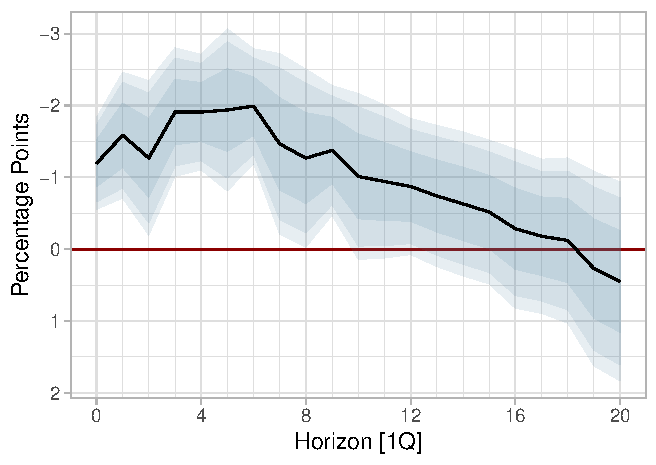
\includegraphics[width=\linewidth]{average_unemployment_long.pdf}
  \end{subfigure}  
  \hfill
  \begin{subfigure}[b]{0.49\textwidth}\centering
    \caption{Differential Resp. to Unemployment Gap}
    \label{fig:LP_long:differential_gap}
    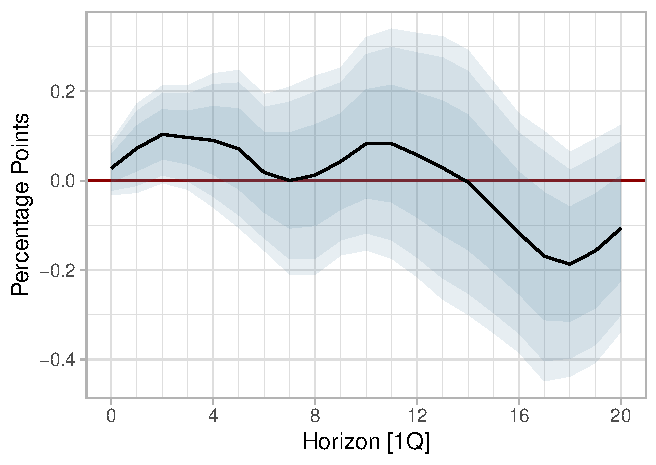
\includegraphics[width=\linewidth]{differential_unemployment_long.pdf}
  \end{subfigure}
      {\begin{flushleft}\scriptsize\textit{Notes}: This figure reports the responses of the $(r-r^*)_t$ to an increase in the Tealbook deflator inflation forecast and $(-)$ unemployment gap forecast of 1 p.p.. The subfigure \ref{fig:LP_long:average_inflation} reports the response of $(r-r^*)_t$ to projected deflator inflation for the $\mathit{HAWK}$ index equal to the sample average; \ref{fig:LP_long:differential_inflation} is the addition to the response in case there are 2 (out of 12 in total) additional consistent hawks in the FOMC. Subfigures \ref{fig:LP_long:average_gap} and \ref{fig:LP_long:differential_gap} report the same for the increase in projected GDP gap for 1p.p. The shaded areas correspond to 68\%, 90\% and 95\% confidence bands calculated with HAC estimator with \citet{Andrews1991} weighting.\end{flushleft}}
\end{minipage}
\end{figure}



\begin{table}[!htbp] \centering \footnotesize
\begin{threeparttable}
  \caption{Estimates of Long LP Taylor Rule} 
  \label{tab:LP_long} 
  \begin{tabular}{@{\extracolsep{5pt}}lccccccc} 
    \\[-1.8ex]\hline 
    \hline \\[-1.8ex] 
    & \multicolumn{7}{c}{\textit{Dependent variable:} $\left(r-r^*\right)_{t+h}$} \\  
    \\[-1.8ex]
    \cline{2-8} 
    \\[-1.8ex] & $h=0$ & $h=2$ & $h=4$ & $h=6$ & $h=8$ & $h=10$ & $h=12$ \\ 
    \\[-1.8ex] & (1) & (2) & (3) & (4) & (5) & (6) & (7)\\ 
    \hline \\[-1.8ex] 
    Expected Deflator   & 0.235 & 0.518$^{**}$ & 0.691$^{*}$ & 0.718 & 0.681 & 0.331 & 0.178 \\ 
    Inflation, $\Delta\mathit{Deflator}_t^e$ & (0.235) & (0.235) & (0.354) & (0.587) & (0.613) & (0.455) & (0.353) \\ 
    & & & & & & & \\ 
    $\quad \times \left(\mathit{Hawk}_t-\overline{\mathit{Hawk}}\right)$ & 0.716 & 1.554$^{**}$ & 2.216$^{***}$ & 3.466$^{***}$ & 2.588$^{**}$ & 1.612 & 0.507 \\ 
    & (0.654) & (0.654) & (0.510) & (1.105) & (1.306) & (1.347) & (1.320) \\ 
    & & & & & & & \\ 
    Expected Unemployment & $-$1.192$^{**}$ & $-$1.268$^{**}$ & $-$1.908$^{***}$ & $-$1.991$^{***}$ & $-$1.267$^{**}$ & $-$1.012$^{*}$ & $-$0.871 \\ 
    Gap, $\left(u-u^*\right)_t^e$ & (0.597) & (0.597) & (0.420) & (0.462) & (0.627) & (0.573) & (0.591) \\ 
    & & & & & & & \\ 
    $\quad \times \left(\mathit{Hawk}_t-\overline{\mathit{Hawk}}\right)$& $-$0.168 & $-$0.621$^{*}$ & $-$0.541 & $-$0.109 & $-$0.074 & $-$0.495 & $-$0.345 \\ 
    & (0.338) & (0.338) & (0.430) & (0.615) & (0.716) & (0.746) & (0.808) \\ 
    & & & & & & & \\ 
    $\left(\mathit{Hawk}_t-\overline{\mathit{Hawk}}\right)$ & $-$1.797 & $-$3.636$^{**}$ & $-$4.432$^{***}$ & $-$6.435$^{**}$ & $-$3.606 & $-$1.688 & 0.305 \\ 
    & (1.477) & (1.477) & (1.431) & (2.614) & (3.186) & (3.162) & (2.740) \\ 
    & & & & & & & \\ 
    \hline \\[-1.8ex] 
    Observations & 200 & 200 & 200 & 200 & 200 & 198 & 196 \\ 
    R$^{2}$ & 0.960 & 0.848 & 0.768 & 0.650 & 0.606 & 0.609 & 0.634 \\ 
    Adjusted R$^{2}$ & 0.956 & 0.833 & 0.746 & 0.618 & 0.569 & 0.572 & 0.600 \\ 
    Residual Std. Error & 0.741 & 1.438 & 1.775 & 2.183 & 2.332 & 2.331 & 2.265 \\ 
    Wu-Hausman & $2.268^{*}$& $6.267^{***}$ & $6.322^{***}$ & $16.09^{***}$ & $9.765^{***}$ & $5.584^{***}$ & $2.04$\\
    \hline 
    \hline
  \end{tabular} 
  \begin{tablenotes}[flushleft]\scriptsize
    \item[] \textit{Notes:} 
    This table reports the estimates of the coefficients of interest in model in \vref{eq:LP1} with projected inflation measured as a projected change in GDP deflator and projected gap is the gap in unemployment. The \citet{Andrews1991} HAC standard errors  are in parenthesis. Weak Instrument statistics (for $h=0$) are the following, hawk: $64.8$; interaction with deflator inflation: $64.2$, interaction with unemployment gap: $79.5$. $^{*}p<0.1$; $^{**}p<0.05$; $^{***}p<0.01$.
  \end{tablenotes}
\end{threeparttable}
\end{table} 




\subsection{Historical Estimates of Size and Persistence}

One of the advantages of using state-dependent local projection framework is that we can look at the fitted values as a predictions of FFR paths made in each period of time. 
The  \vref{fig:pathes_predictions} shows the point-predictions made using the model \vref{eq:LP1} based on the FOMC composition and tealbook projections of inflation and output gap. I restrict the prediction horizon to 16 quarters, which represent the 

The predicted pathes are hard to analyze, so one of the ways to look at them\footnote{Which is inspired by the size-persistence tradeoff in heterogeneous agent new keynesian model (HANK) by \cite{KMV2018}} is to estimate the size and persistence of monetary policy. Deviating from \cite{KMV2018} the size is defined as a mean of predicted rate path 



\begin{figure}[!htbp]\centering
  \begin{minipage}{1\textwidth}\centering
    \caption{Predictions of FFR Paths Made in Each of the Period.} 
    \label{fig:pathes_predictions}
    \vspace{2ex}
    \begin{subfigure}[b]{0.495\textwidth}\centering
      \caption{Short Specification}
      \label{fig:pathes_predictions_short}
      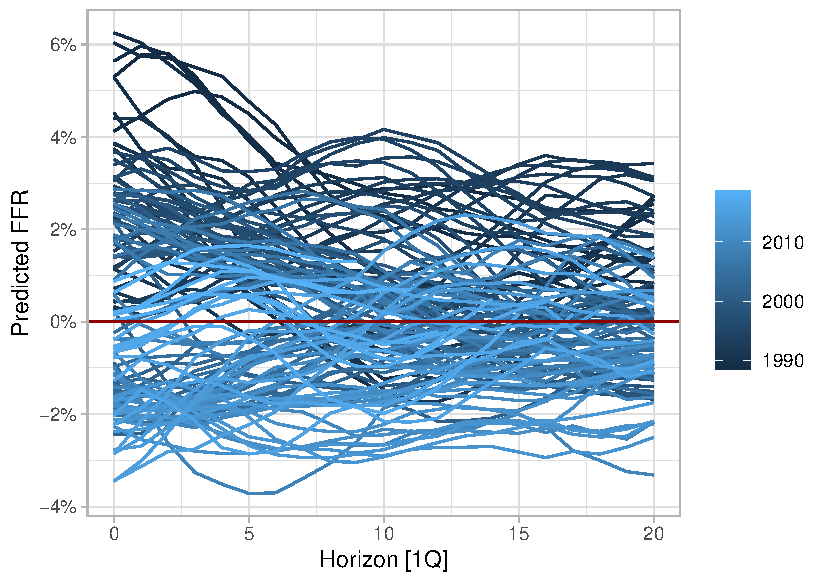
\includegraphics[width=\linewidth]{predicted_paths_short.pdf}
    \end{subfigure}\hfill
    \begin{subfigure}[b]{0.495\textwidth}\centering
      \caption{Long Specification}
      \label{fig:pathes_predictions_long}
      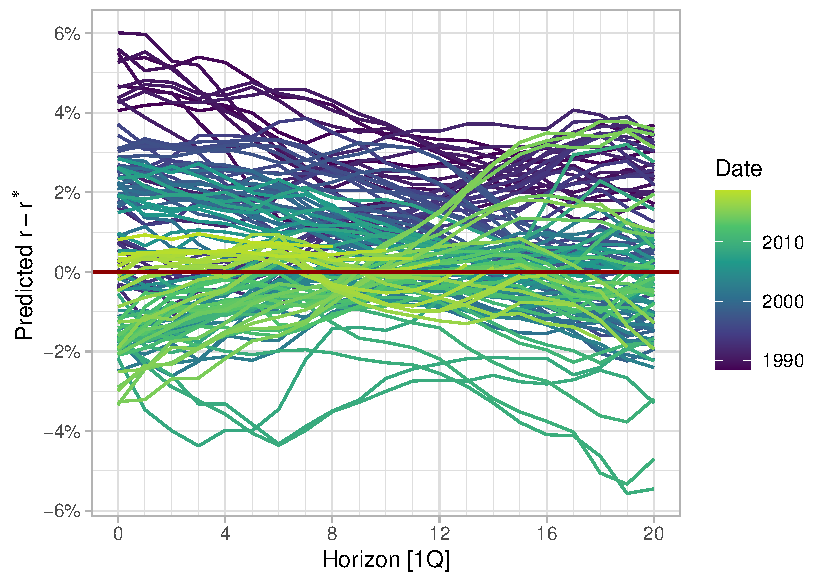
\includegraphics[width=\linewidth]{predicted_paths_long.pdf}
    \end{subfigure}
    {\begin{flushleft}
      \scriptsize \textit{Notes:} This figure shows the \vref{eq:LP1} model predictions of FFR rate paths made in each period of time for 2 specifications. The prediction period is restricted to start at 1988 Q3 for both specifications.
    \end{flushleft}} 
    \end{minipage}

\end{figure}



\begin{figure}[!hpbt]\centering
  \begin{minipage}{1\textwidth}\centering
    \caption{Historical Estimates of Size and Persistence} 
    \label{fig:size_persistence}
    \vspace{1ex}
    \begin{subfigure}[b]{0.5\textwidth}\centering
      \caption{Short Specification}
      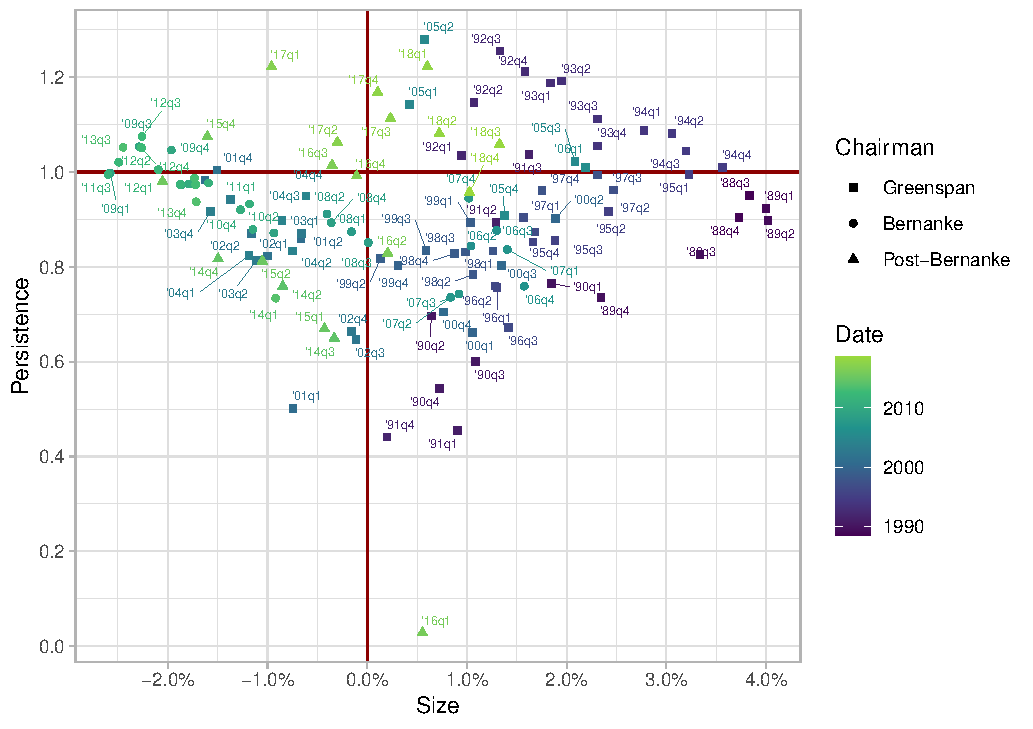
\includegraphics[width=\linewidth]{actual_size_persistence_short.pdf}
    \end{subfigure}\hfill
    \begin{subfigure}[b]{0.5\textwidth}\centering
      \caption{Long Specification}
      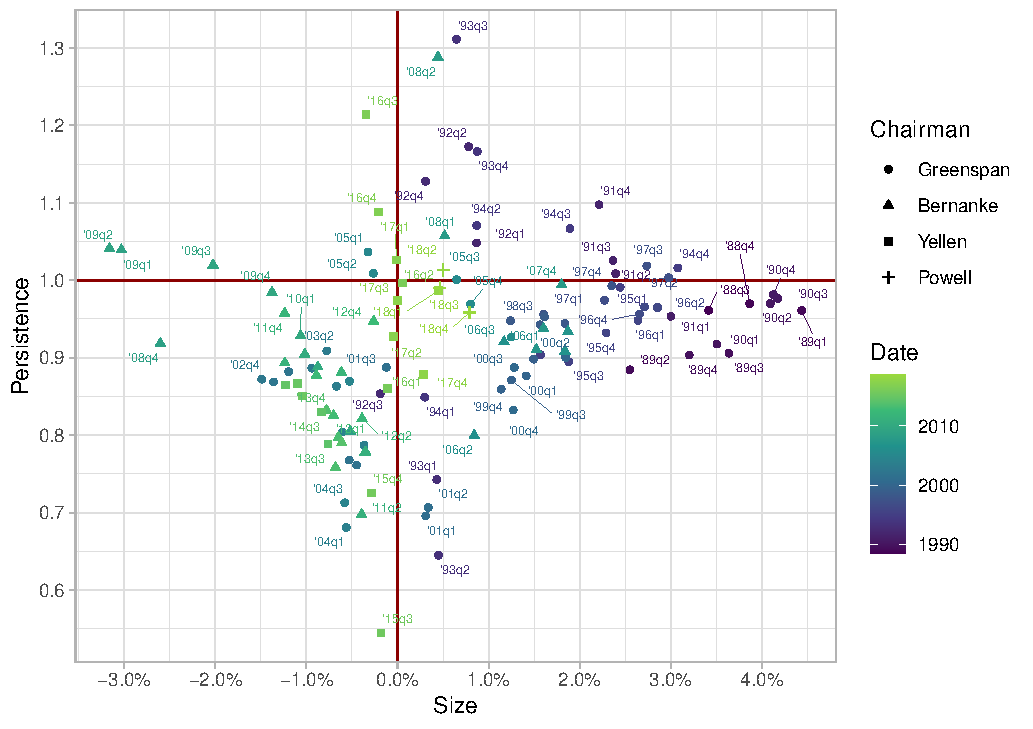
\includegraphics[width=\linewidth]{actual_size_persistence_long.pdf}
    \end{subfigure}
    {\begin{flushleft}\scriptsize \textit{Notes:} This figure shows the size and persistence calculated as in for 2 specifications. The prediction period is restricted to start at 1988 Q3 for both specifications.\end{flushleft}} 
    \end{minipage}
    
\end{figure}


% Based on the impulse responses above I restrict the horizon for the size and persistence calculation to the 8th quarter, i.e. in equation \eqref{eq:pred_policy} I set $H$ to be equal to 8. The estimates of coefficients of the models \vref{eq:linear,eq:quadratic} can be seen in \vref{tab:Size-Persistence}.




% \begin{table}[!htb] \centering \footnotesize
%     \begin{threeparttable}
%     \caption{Size-Persistence Tradeoff} 
%     \label{tab:Size-Persistence} 
%     \begin{tabular}{@{\extracolsep{10pt}}lcc} 
%       \\[-1.8ex]\hline 
%       \hline \\[-1.8ex] 
%        & \multicolumn{2}{c}{\textit{Dependent variable:}} \\ 
%       \cline{2-3} 
%       \\[-1.8ex] & \multicolumn{2}{c}{$\log(\mathit{consumption})$} \\  \\[-1.8ex]   &\multicolumn{2}{c}{$H=8$}\\
%       \\[-1.8ex] & (1) & (2)\\ 
%       \hline \\[-1.8ex] 
%        Size $(R_0)$  & $-$0.687 & $-$0.451 \\ 
%         & ($-$1.149, $-$0.133) & ($-$1.495, 1.078)    \\ 
%         &[0.011]\{0.997\} & [0.857]\{0.578\}\\ 
%         & & \\ 
%        Persistence $(\nu)$ & $-$0.100 & 1.223 \\ 
%         & ($-$0.693,  0.691)   & ($-$3.598, 4.968)    \\ 
%         &[0.746]\{0.673\} & [0.517]\{0.246\}\\ 
%         & & \\ 
%         $\nu^2$ &  & $-$1.042 \\ 
%         &  &  ($-$4.271, 4.336) \\ 
%         & &[0.517]\{0.766\} \\ 
%         & & \\ 
%        $R_0\times \nu$ & 0.765 & $-$1.628 \\ 
%         & ($-$0.177,  1.526)    &   ($-$3.159,  2.748)     \\ 
%         &[0.0754]\{0.0247\} & [0.522]\{0.759\}\\ 
%         & & \\ 
%         $R_0\times \nu^2$ &  & 2.435 \\ 
%         &  &  ($-$1.852, 3.838) \\ 
%         & & [0.340]\{0.145\}\\ 
%         & & \\ 
%        Constant & 10.6 &10.5 \\ 
%         & (10.1, 11.0) & (9.8, 11.0)    \\ 
%         & [0.0]\{0.0\}& [0.0]\{0.0\}\\ 
%         & & \\[-1.8ex] 
%       \hline \\[-1.8ex] 
%       Observations & 198 & 198 \\ 
%       R$^{2}$ & 0.338 & 0.343 \\ 
%       Adjusted R$^{2}$ & 0.328 & 0.326 \\ 
%       \hline 
%       \hline \\[-1.8ex] 
%       \end{tabular} 
%     \begin{tablenotes}[flushleft]
%     \item[] \scriptsize \textit{Note:} The inference is derived from Block bootstrap with 10,000 replications and block lengths geometrically distributed with mean $16$. 95\% percentile intervals are in parenthesis. Bootstrap p-values for the two-sided hypothesis ($\mathbb{H}_0:\theta=0$ vs $\mathbb{H}_a:\theta\ne 0$) are in square brackets, p-values for the one-sided hypothesis ($\mathbb{H}_0:\theta=0$ vs $\mathbb{H}_a:\theta>0$) are in curly brackets. 
%   \end{tablenotes}
% \end{threeparttable}
%   \end{table} 








% \begin{figure}[!htbp]\centering
%   \caption{Size and Persistence Dynamics}
%   \vspace{2ex}
%   \label{fig:Size_Persistence_Dynamics}
%   \begin{subfigure}[b]{0.495\textwidth}
%       \centering
%       \caption{Size Dynamics}
%       \label{fig:size}
%       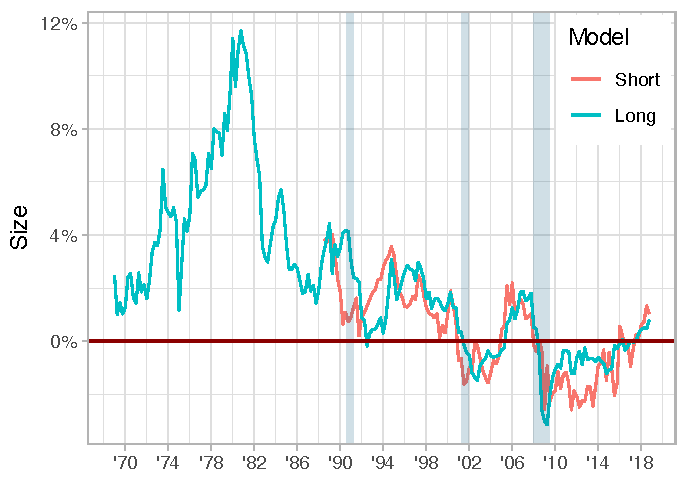
\includegraphics[width=\linewidth]{size_plot.pdf}
%   \end{subfigure}
%   \hfill
%   \begin{subfigure}[b]{0.495\textwidth}
%       \centering
%       \caption{Persistence Dynamics}
%       \label{fig:DifferentialResponce}
%       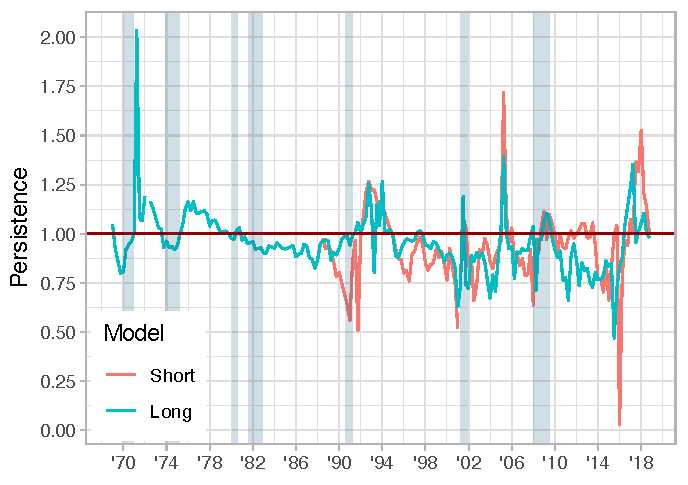
\includegraphics[width=\linewidth]{persistence_plot.pdf}
%   \end{subfigure}
%       {\begin{flushleft}\scriptsize\textit{Notes}: This figure presents the size and persistence, calculated as mean and the first autocorrelation of impulse-response function in each state, constructed as described in , over time. \end{flushleft}}
% \end{figure}







% \section{Robustness}
% tba






\newpage~
\bibliography{../misc/references.bib}
\bibliographystyle{../misc/econ}
\newpage
\appendix

\numberwithin{equation}{section}
\numberwithin{table}{section}
\numberwithin{figure}{section}



\section{Appendix. Data sources} 


\noindent\textbf{HAWK and HAWK IV Indexes.} \citet{Istrefi2019} classifies each FOMC member as hawk or dove based on more than 20,000 historical media articles.\citet{Istrefi2019} categorizes FOMC member for each FOMC meeting based on the news information available up to the meeting. Hawks are perceived to be more concerned about inflation, while doves are more concerned with employment and growth. \citet{BordoIstrefi2023} show that educational background (Freshwater vs. Saltwater) and crises experience of FOMC member predict their policy preferences.

\citet{HIM2023} aggregate this classification as follows. First, they define the policy preferences of each FOMC member $i$ at meeting $\tau$, $\mathit{Hawk}_{i\tau}$, as 
\[\textit{Hawk}_{i\tau}=\begin{cases}
  +1&\text{Consistent hawk}\\
  +\frac{1}{2}&\text{Swinging hawk}\\ ~~\, 0&\text{Preference unknown}\\ 
  -\frac{1}{2}&\text{Swinging dove}\\ 
  -1&\text{Consistent dove}
\end{cases}.\]
A consistent hawk is a member that has not been categorized as a dove previously, in contrast a swinging hawk is a member that was a dove before. Then the hawkishness of the bord at meeting $\tau$ is the average of the members present, that is
\[\textit{Hawk}_{\tau}=\frac{1}{\left|\mathcal{M}_\tau\right|}\sum_{i\in \mathcal{M}_\tau}\textit{Hawk}_{i\tau}.\]
Then $\textit{Hawk}_{\tau}$ is aggregated to the quarterly level into $\mathit{Hawk}_t$, which is used in this work.

$\mathit{Hawk}_t^\mathit{IV}$ is constructed the similar way but on the portion of the FOMC memberships that is rotated each year. Each year 4/12 FOMC memberships rotate among 11 FRB presidents (Cleveland and Chicago get a seat every second year and Philadelphia, Richmond, Boston, Dallas, Atlanta, St. Louis, Minneapolis, San Francisco, Kansas City -- every third year) and this rotation is independent of cycle.

\noindent\textbf{Federal Funds Rate.}
To measure $r_t$ I take the minimum of the effective federal funds rate (DFF) and shadow federal funds rate by \citet{WuXia2016}. This approach allows me to deal the zero lower bound episode and have a measure of the the estimate by \citet{WuXia2016} to periods earlier than (1990 Q1) zero lower bound episodes. 

\noindent\textbf{Natural Rate Estimates.}
Natural rate of interest used is estimated by \citet{LW2003} and re-estimated by \citet{HLW2023} to bridge the Covid period.

\noindent\textbf{Tealbook Projections.}  



\newpage
\section{Appendix. Regression Tables}

\begin{table}[!htbp] \centering \scriptsize
    \begin{threeparttable}
    \caption{Estimates of Short LP Taylor Rule} 
    \label{tab:LP_short_full} 
    \begin{tabular}{@{\extracolsep{3pt}}lccccccc} 
      \\[-1.8ex]\hline 
      \hline \\[-1.8ex] 
       & \multicolumn{7}{c}{\textit{Dependent variable:} $\left(r-r^*\right)_{t+h}$} \\ 
       \\[-1.8ex] 
      \cline{2-8} 
      \\[-1.8ex] & $h=0$ & $h=2$ & $h=4$ & $h=6$ & $h=8$ & $h=10$ & $h=12$ \\ 
      \\[-1.8ex] & (1) & (2) & (3) & (4) & (5) & (6) & (7)\\ 
      \hline \\[-1.8ex] 
       Expected CPI Inflation, $\Delta\mathit{CPI}_t^e$ & 0.175$^{**}$ & 0.570$^{***}$ & 0.923$^{***}$ & 0.856$^{***}$ & 0.791$^{***}$ & 0.738$^{**}$ & 0.596 \\ 
       & (0.073) & (0.157) & (0.263) & (0.308) & (0.281) & (0.342) & (0.448) \\ 
        & & & & & & & \\ 
        $\quad \times \left(\mathit{Hawk}_t-\overline{\mathit{Hawk}}\right)$ & 0.170 & $-$0.191 & $-$1.600$^{**}$ & $-$2.224$^{**}$ & $-$1.741 & $-$2.091$^{*}$ & $-$2.070 \\ 
        & (0.186) & (0.530) & (0.749) & (1.094) & (1.122) & (1.193) & (1.473) \\ 
        & & & & & & & \\ 
       Expected GDP Gap, $x_{t}^e$ & 0.177$^{***}$ & 0.483$^{***}$ & 0.709$^{***}$ & 0.815$^{***}$ & 0.733$^{***}$ & 0.653$^{**}$ & 0.633$^{*}$ \\ 
       & (0.058) & (0.180) & (0.157) & (0.160) & (0.176) & (0.271) & (0.325) \\ 
        & & & & & & & \\ 
       $\quad \times \left(\mathit{HAWK}-\overline{\mathit{HAWK}}\right)_t$ & 0.089$^{*}$ & 0.158 & 0.002 & $-$0.122 & $-$0.013 & 0.217 & 0.263 \\ 
       & (0.046) & (0.156) & (0.244) & (0.302) & (0.320) & (0.308) & (0.403) \\ 
       & & & & & & & \\ 
    $\left(\mathit{HAWK}-\overline{\mathit{HAWK}}\right)_t$ & $-$0.146 & 0.875 & 3.991$^{*}$ & 6.539$^{**}$ & 7.241$^{**}$ & 8.725$^{**}$ & 7.998$^{**}$ \\ 
    & (0.446) & (1.321) & (2.151) & (3.167) & (3.432) & (3.640) & (3.928) \\ 
      & & & & & & & \\ 
      $\left(r-r^*\right)_{t-1}$ & 1.308$^{***}$ & 1.454$^{***}$ & 0.962$^{***}$ & 0.423 & $-$0.050 & $-$0.464 & $-$0.938 \\ 
      & (0.143) & (0.302) & (0.351) & (0.415) & (0.443) & (0.551) & (0.685) \\ 
      & & & & & & & \\ 
      $\left(r-r^*\right)_{t-2}$ & $-$0.274 & $-$0.666$^{***}$ & $-$0.548 & $-$0.050 & 0.336 & 0.220 & 0.263 \\ 
      & (0.207) & (0.231) & (0.342) & (0.391) & (0.394) & (0.520) & (0.580) \\ 
      & & & & & & & \\ 
      $\left(r-r^*\right)_{t-3}$ & $-$0.244 & $-$0.458$^{***}$ & $-$0.059 & 0.030 & $-$0.036 & 0.148 & 0.328 \\ 
      & (0.156) & (0.177) & (0.306) & (0.365) & (0.377) & (0.376) & (0.385) \\ 
      & & & & & & & \\ 
      $\left(r-r^*\right)_{t-4}$ & 0.031 & 0.145 & $-$0.172 & $-$0.612 & $-$0.990$^{***}$ & $-$1.140$^{***}$ & $-$1.076$^{**}$ \\ 
      & (0.098) & (0.236) & (0.346) & (0.376) & (0.358) & (0.441) & (0.503) \\ 
      & & & & & & & \\ 
    $\Delta\mathit{CPI}_{t-1}^e$ & 0.005 & 0.093 & $-$0.005 & 0.076 & 0.089 & 0.170 & 0.290 \\ 
    & (0.071) & (0.101) & (0.137) & (0.172) & (0.163) & (0.228) & (0.241) \\ 
      & & & & & & & \\ 
      $\Delta\mathit{CPI}_{t-2}^e$ & 0.057 & 0.184 & 0.030 & $-$0.062 & 0.005 & 0.177 & 0.340 \\ 
      & (0.084) & (0.188) & (0.287) & (0.320) & (0.351) & (0.357) & (0.355) \\ 
      & & & & & & & \\ 
      $\Delta\mathit{CPI}_{t-3}^e$ & 0.134$^{*}$ & 0.084 & 0.181 & 0.249 & 0.270 & 0.433 & 0.459$^{*}$ \\ 
      & (0.069) & (0.128) & (0.187) & (0.255) & (0.274) & (0.277) & (0.236) \\ 
      & & & & & & & \\ 
      $\Delta\mathit{CPI}_{t-4}^e$ & $-$0.077 & $-$0.127 & $-$0.007 & 0.200 & 0.575$^{***}$ & 0.901$^{***}$ & 1.183$^{***}$ \\ 
      & (0.056) & (0.121) & (0.184) & (0.168) & (0.173) & (0.248) & (0.273) \\ 
      & & & & & & & \\ 
      $x_{t-1}^e$ & $-$0.057 & $-$0.208 & $-$0.340$^{*}$ & $-$0.567$^{***}$ & $-$0.529$^{**}$ & $-$0.494$^{**}$ & $-$0.412$^{*}$ \\ 
      & (0.089) & (0.166) & (0.183) & (0.181) & (0.231) & (0.238) & (0.243) \\ 
      & & & & & & & \\ 
      $x_{t-2}^e$ & $-$0.102 & $-$0.064 & 0.107 & 0.268 & 0.251 & 0.417$^{**}$ & 0.371$^{*}$ \\ 
      & (0.074) & (0.127) & (0.194) & (0.229) & (0.212) & (0.202) & (0.224) \\ 
      & & & & & & & \\ 
      $x_{t-3}^e$  & 0.044 & $-$0.023 & $-$0.427$^{**}$ & $-$0.644$^{**}$ & $-$0.669$^{*}$ & $-$0.715 & $-$0.704 \\ 
      & (0.099) & (0.118) & (0.191) & (0.286) & (0.354) & (0.449) & (0.488) \\ 
      & & & & & & & \\ 
      $x_{t-4}^e$ & 0.022 & $-$0.010 & 0.072 & 0.182 & 0.326 & 0.378 & 0.427 \\ 
      & (0.062) & (0.112) & (0.202) & (0.240) & (0.240) & (0.275) & (0.311) \\ 
      & & & & & & & \\ 
    Constant & $-$0.546$^{**}$ & $-$1.428$^{**}$ & $-$1.829 & $-$1.944 & $-$2.587 & $-$3.800$^{**}$ & $-$4.825$^{**}$ \\ 
    & (0.219) & (0.666) & (1.174) & (1.614) & (1.801) & (1.907) & (2.002) \\ 
      & & & & & & & \\ 
      \hline \\[-1.8ex] 
      Observations & 122 & 122 & 122 & 122 & 122 & 120 & 118 \\ 
      R$^{2}$ & 0.983 & 0.912 & 0.784 & 0.647 & 0.528 & 0.416 & 0.373 \\ 
      Adjusted R$^{2}$ & 0.981 & 0.898 & 0.749 & 0.590 & 0.451 & 0.318 & 0.266 \\ 
      Residual Std. Error & 0.322 & 0.716 & 1.063 & 1.295 & 1.457 & 1.582 & 1.622 \\
      Wu-Hausman & 0.395& 0.352& 0.718& 1.891& $6.496^{***}$ &$15.97^{***}$& $15.05^{***}$ \\
      \hline 
      \hline
      \end{tabular} 
  \begin{tablenotes}[flushleft]\scriptsize
\item[] \textit{Notes:} This table reports the estimates of the coefficients of interest in model in \vref{eq:LP1} with projected inflation measured as a projected change in CPI. The \citet{Andrews1991} HAC standard errors are in parenthesis. Weak Instrument statistics (for $h=0$) are HAWK: $53.5$; interaction with CPI inflation: $42.2$, interaction with GDP gap: $51.4$. $^{*}p<0.1$; $^{**}p<0.05$; $^{***}p<0.01$.
\end{tablenotes}
\end{threeparttable}
  \end{table} 

  \begin{table}[!htbp] \centering \scriptsize
    \begin{threeparttable}
    \caption{First Stage of the Short LP Model} 
    \label{tab:fs_short} 
  \begin{tabular}{@{\extracolsep{5pt}}lccc} 
  \\[-1.8ex]\hline 
  \hline \\[-1.8ex] 
   & \multicolumn{3}{c}{\textit{Dependent variable:}} \\ 
  \cline{2-4} 
  \\[-1.8ex] & $\left(\mathit{Hawk}_t-\overline{\mathit{Hawk}}\right)$ &  $\times \mathit{CPI}_t^e$ & $\times x_{t}$ \\ 
  \\[-1.8ex] & (1) & (2) & (3)\\ 
  \hline \\[-1.8ex] 
  Expected CPI Inflation, $\Delta\mathit{CPI}_t^e$ & 0.017 & 0.057 & 0.127$^{**}$ \\ 
    & (0.034) & (0.084) & (0.055) \\ 
    & & & \\ 
    $\quad\times\left(\mathit{HAWK}^\mathit{IV}-\overline{\mathit{HAWK}}^\mathit{IV}\right)_t$ & $-$0.124$^{***}$ & 0.144 & $-$0.168$^{**}$ \\ 
    & (0.044) & (0.109) & (0.071) \\ 
    & & & \\ 
    Expected GDP Gap, $x_{t}^e$  & 0.022 & 0.039 & 0.032 \\ 
    & (0.028) & (0.070) & (0.046) \\ 
    & & & \\ 
    $\quad\times\left(\mathit{HAWK}^\mathit{IV}-\overline{\mathit{HAWK}}^\mathit{IV}\right)_t$ & 0.031$^{**}$ & 0.030 & $-$0.258$^{***}$ \\ 
    & (0.016) & (0.038) & (0.025) \\ 
    & & & \\ 
   $\left(\mathit{HAWK}^\mathit{IV}-\overline{\mathit{HAWK}}^\mathit{IV}\right)_t$ & 0.776$^{***}$ & 0.779$^{***}$ & 0.408$^{**}$ \\ 
    & (0.108) & (0.267) & (0.175) \\ 
    & & & \\ 

    $\left(r-r^*\right)_{t-1}$ & 0.041 & $-$0.018 & $-$0.125 \\ 
    & (0.052) & (0.128) & (0.084) \\ 
    & & & \\ 
    $\left(r-r^*\right)_{t-1}$ & $-$0.013 & 0.003 & 0.030 \\ 
    & (0.082) & (0.203) & (0.133) \\ 
    & & & \\ 
    $\left(r-r^*\right)_{t-1}$ & $-$0.041 & 0.081 & $-$0.062 \\ 
    & (0.082) & (0.203) & (0.133) \\ 
    & & & \\ 
    $\left(r-r^*\right)_{t-1}$ & 0.090$^{*}$ & 0.061 & $-$0.021 \\ 
    & (0.048) & (0.118) & (0.077) \\ 
    & & & \\ 
    $\Delta\mathit{CPI}_{t-1}^e$ & $-$0.002 & 0.037 & 0.110$^{*}$ \\ 
    & (0.038) & (0.093) & (0.061) \\ 
    & & & \\ 
    $\Delta\mathit{CPI}_{t-2}^e$  & 0.047 & 0.052 & 0.140$^{**}$ \\ 
    & (0.039) & (0.095) & (0.062) \\ 
    & & & \\ 
    $\Delta\mathit{CPI}_{t-3}^e$  & 0.011 & 0.066 & 0.070 \\ 
    & (0.037) & (0.091) & (0.059) \\ 
    & & & \\ 
    $\Delta\mathit{CPI}_{t-4}^e$  & 0.014 & 0.092 & 0.056 \\ 
    & (0.033) & (0.081) & (0.053) \\ 
    & & & \\ 
   $x_{t-1}^e$ & $-$0.016 & $-$0.051 & $-$0.016 \\ 
    & (0.047) & (0.116) & (0.076) \\ 
    & & & \\ 
    $x_{t-2}^e$ & $-$0.007 & 0.053 & 0.044 \\ 
    & (0.045) & (0.112) & (0.073) \\ 
    & & & \\ 
    $x_{t-3}^e$ & 0.002 & $-$0.087 & $-$0.042 \\ 
    & (0.043) & (0.107) & (0.070) \\ 
    & & & \\ 
    $x_{t-4}^e$ & 0.004 & 0.015 & 0.126$^{***}$ \\ 
    & (0.030) & (0.073) & (0.048) \\ 
    & & & \\ 

   Constant & $-$0.340$^{***}$ & $-$0.843$^{***}$ & $-$1.058$^{***}$ \\ 
    & (0.076) & (0.188) & (0.123) \\ 
    & & & \\ 
  \hline \\[-1.8ex] 
  Observations & 122 & 122 & 122 \\ 
  R$^{2}$ & 0.857 & 0.814 & 0.866 \\ 
  Adjusted R$^{2}$ & 0.833 & 0.783 & 0.844 \\ 
  Residual Std. Error & 0.162 & 0.399 & 0.261 \\ 
  F Statistic & 36.591$^{***}$ & 26.699$^{***}$ & 39.550$^{***}$ \\
  Weak instrument F & 53.576 & 42.241 & 51.408 \\
  \hline 
  \hline
\end{tabular} 
  \begin{tablenotes}[flushleft]
    \item[]\textit{Notes:} The \citet{Andrews1991} HAC standard errors are in parenthesis. $^{*}p<0.1$; $^{**}p<0.05$; $^{***}p<0.01$.
  \end{tablenotes}
\end{threeparttable}
  \end{table} 

  \begin{table}[!htbp] \centering \scriptsize
    \begin{threeparttable}
    \caption{Estimates of Long LP Taylor Rule} 
    \label{} 
  \begin{tabular}{@{\extracolsep{5pt}}lccccccc} 
  \\[-1.8ex]\hline 
  \hline \\[-1.8ex] 
  & \multicolumn{7}{c}{\textit{Dependent variable:} $\left(r-r^*\right)_{t+h}$} \\ \\[-1.8ex] 
  \cline{2-8} 
  \\[-1.8ex] & $h=0$ & $h=2$ & $h=4$ & $h=6$ & $h=8$ & $h=10$ & $h=12$ \\ 
  \\[-1.8ex] & (1) & (2) & (3) & (4) & (5) & (6) & (7)\\ 
  \hline \\[-1.8ex] 
  Expected Deflator Inflation,  & 0.235 & 0.518$^{**}$ & 0.691$^{*}$ & 0.718 & 0.681 & 0.331 & 0.178 \\ 
  $\Delta\mathit{Deflator}_t^e$ & (0.235) & (0.235) & (0.354) & (0.587) & (0.613) & (0.455) & (0.353) \\ 
    & & & & & & & \\ 
   $\quad \times \left(\mathit{Hawk}_t-\overline{\mathit{Hawk}}\right)$ & 0.716 & 1.554$^{**}$ & 2.216$^{***}$ & 3.466$^{***}$ & 2.588$^{**}$ & 1.612 & 0.507 \\ 
    & (0.654) & (0.654) & (0.510) & (1.105) & (1.306) & (1.347) & (1.320) \\ 
    & & & & & & & \\ 
   Expected Unemployment Gap, & $-$1.192$^{**}$ & $-$1.268$^{**}$ & $-$1.908$^{***}$ & $-$1.991$^{***}$ & $-$1.267$^{**}$ & $-$1.012$^{*}$ & $-$0.871 \\ 
    $\left(u-u^*\right)_t$ & (0.597) & (0.597) & (0.420) & (0.462) & (0.627) & (0.573) & (0.591) \\ 
    & & & & & & & \\ 
    $\quad \times \left(\mathit{Hawk}_t-\overline{\mathit{Hawk}}\right)$& $-$0.168 & $-$0.621$^{*}$ & $-$0.541 & $-$0.109 & $-$0.074 & $-$0.495 & $-$0.345 \\ 
    & (0.338) & (0.338) & (0.430) & (0.615) & (0.716) & (0.746) & (0.808) \\ 
    & & & & & & & \\ 
    $\left(\mathit{Hawk}_t-\overline{\mathit{Hawk}}\right)$ & $-$1.797 & $-$3.636$^{**}$ & $-$4.432$^{***}$ & $-$6.435$^{**}$ & $-$3.606 & $-$1.688 & 0.305 \\ 
    & (1.477) & (1.477) & (1.431) & (2.614) & (3.186) & (3.162) & (2.740) \\ 
    & & & & & & & \\ 
    $\left(r-r^*\right)_{t-1}$ & 1.005$^{***}$ & 0.485$^{***}$ & 0.485$^{**}$ & $-$0.056 & 0.043 & $-$0.355$^{*}$ & $-$0.416$^{**}$ \\ 
    & (0.176) & (0.176) & (0.208) & (0.232) & (0.184) & (0.186) & (0.177) \\ 
    & & & & & & & \\ 
    $\left(r-r^*\right)_{t-2}$ & $-$0.169 & 0.146 & 0.101 & 0.466$^{***}$ & 0.261 & 0.198$^{**}$ & 0.088 \\ 
    & (0.202) & (0.202) & (0.212) & (0.166) & (0.210) & (0.085) & (0.229) \\ 
    & & & & & & & \\ 
    $\left(r-r^*\right)_{t-3}$ & 0.147 & 0.411$^{**}$ & 0.024 & 0.273$^{*}$ & $-$0.186 & $-$0.071 & $-$0.186 \\ 
    & (0.180) & (0.180) & (0.146) & (0.162) & (0.199) &  & (0.161) \\ 
    & & & & & & & \\ 
    $\left(r-r^*\right)_{t-4}$ & 0.054 & $-$0.113 & 0.168 & $-$0.030 & 0.171 & 0.195 & 0.208 \\ 
    & (0.160) & (0.160) & (0.216) & (0.259) & (0.291) & (0.311) & (0.281) \\ 
    & & & & & & & \\ 
    $\Delta\mathit{Deflator}_{t-1}^e$ & 0.038 & 0.157 & $-$0.116 & 0.030 & $-$0.367 & $-$0.019 & $-$0.0005 \\ 
    & (0.196) & (0.196) & (0.215) & (0.240) & (0.377) & (0.252) & (0.334) \\ 
    & & & & & & & \\ 
    $\Delta\mathit{Deflator}_{t-2}^e$ & $-$0.138 & $-$0.160 & $-$0.052 & $-$0.155 & 0.042 & 0.107 & 0.323$^{**}$ \\ 
    & (0.367) & (0.367) & (0.221) & (0.256) & (0.311) & (0.216) & (0.161) \\ 
    & & & & & & & \\ 
    $\Delta\mathit{Deflator}_{t-3}^e$ & 0.109 & $-$0.410 & $-$0.237 & $-$0.814$^{**}$ & $-$0.337 & $-$0.176 & 0.150 \\ 
    & (0.262) & (0.262) & (0.277) & (0.358) & (0.306) & (0.262) & (0.104) \\ 
    & & & & & & & \\ 
    $\Delta\mathit{Deflator}_{t-4}^e$ & $-$0.346 & $-$0.143 & $-$0.357 & $-$0.112 & 0.194 & 0.708$^{**}$ & 0.917$^{***}$ \\ 
    & (0.247) & (0.247) & (0.413) & (0.419) & (0.371) & (0.344) & (0.354) \\ 
    & & & & & & & \\ 
   $\left(u-u^*\right)_{t-1}$ & 1.220 & 0.244 & 1.011$^{**}$ & 0.763 & 0.088 & $-$0.269 & $-$0.244 \\ 
    & (0.799) & (0.799) & (0.441) & (0.639) & (1.096) & (1.009) & (0.780) \\ 
    & & & & & & & \\ 
    $\left(u-u^*\right)_{t-2}$ & 0.057 & 0.248 & $-$0.074 & 0.589 & 0.779 & 0.289 & 0.029 \\ 
    & (0.178) & (0.178) & (0.320) & (0.572) & (0.882) & (0.569) & (0.491) \\ 
    & & & & & & & \\ 
    $\left(u-u^*\right)_{t-3}$ & $-$0.615$^{*}$ & 0.474 & 0.963$^{*}$ & 0.847 & 0.088 & 0.190 & 0.180 \\ 
    & (0.320) & (0.320) & (0.510) & (0.722) & (0.728) & (0.523) & (0.620) \\ 
    & & & & & & & \\ 
    $\left(u-u^*\right)_{t-4}$ & 0.333 & $-$0.138 & $-$0.448 & $-$0.626 & 0.045 & 0.396 & 0.558 \\ 
    & (0.298) & (0.298) & (0.569) & (0.676) & (0.582) & (0.484) & (0.597) \\ 
    & & & & & & & \\ 

  
   Constant & 0.082 & $-$0.111 & 0.051 & 0.663 & $-$0.095 & $-$1.352 & $-$2.355$^{**}$ \\ 
    & (0.555) & (0.555) & (0.656) & (0.968) & (1.074) & (1.174) & (1.090) \\ 
    & & & & & & & \\ 
  \hline \\[-1.8ex] 
  Observations & 200 & 200 & 200 & 200 & 200 & 198 & 196 \\ 
  R$^{2}$ & 0.960 & 0.848 & 0.768 & 0.650 & 0.606 & 0.609 & 0.634 \\ 
  Adjusted R$^{2}$ & 0.956 & 0.833 & 0.746 & 0.618 & 0.569 & 0.572 & 0.600 \\ 
  Residual Std. Error & 0.741 & 1.438 & 1.775 & 2.183 & 2.332 & 2.331 & 2.265 \\ 
  Wu-Hausman & $2.268^{*}$& $6.267^{***}$ & $6.322^{***}$ & $16.09^{***}$ & $9.765^{***}$ & $5.584^{***}$ & $2.04$\\
  \hline 
  \hline
  \end{tabular} 
  \begin{tablenotes}[flushleft]
    \item[] \textit{Notes:} The \citet{Andrews1991} HAC standard errors are in parenthesis. Weak Instrument statistics (for $h=0$) are HAWK: $64.8$; interaction with deflator inflation: $64.2$, interaction with unemployment gap: $79.5$. $^{*}p<0.1$; $^{**}p<0.05$; $^{***}p<0.01$.
  \end{tablenotes}
\end{threeparttable}
    \end{table} 


    \begin{table}[!htbp] \centering \scriptsize 
      \begin{threeparttable}
      \caption{First-Stage of the Long LP Model} 
      \label{tab:fs_long} 
    \begin{tabular}{@{\extracolsep{5pt}}lccc} 
    \\[-1.8ex]\hline 
    \hline \\[-1.8ex] 
    & \multicolumn{3}{c}{\textit{Dependent variable:}} \\ 
    \cline{2-4} 
    \\[-1.8ex] & $\left(\mathit{Hawk}_t-\overline{\mathit{Hawk}}\right)$ &  $\times \Delta\mathit{Deflator}_t^e$ & $\times (u-u^*)_{t}$ \\ 
    \\[-1.8ex] & (1) & (2) & (3)\\ 
    \hline \\[-1.8ex] 
    Expected Deflator Inflation, & $-$0.008 & $-$0.024 & $-$0.053 \\ 
    $\Delta\mathit{Deflator}_t^e$ & (0.031) & (0.080) & (0.047) \\ 
      & & & \\ 
    $\quad \times \left(\mathit{Hawk}_t^\mathit{IV}-\overline{\mathit{Hawk}}^\mathit{IV}\right)$& $-$0.081$^{***}$ & 0.169$^{***}$ & $-$0.010 \\ 
      & (0.020) & (0.053) & (0.031) \\ 
      & & & \\ 
    $(u-u^*)_{t}$ & $-$0.027 & $-$0.091 & $-$0.089 \\ 
    & (0.046) & (0.120) & (0.070) \\ 
    & & & \\ 
    $\quad \times \left(\mathit{Hawk}_t^\mathit{IV}-\overline{\mathit{HAWK}}^\mathit{IV}\right)$& $-$0.094$^{***}$ & $-$0.160$^{***}$ & 0.481$^{***}$ \\ 
    & (0.021) & (0.054) & (0.031) \\ 
    & & & \\ 
    $\left(\mathit{Hawk}_t^\mathit{IV}-\overline{\mathit{Hawk}}^\mathit{IV}\right)$ & 0.703$^{***}$ & 0.785$^{***}$ & $-$0.023 \\ 
    & (0.067) & (0.174) & (0.101) \\ 
    & & & \\ 
    $\left(r-r^*\right)_{t-1}$ & $-$0.007 & $-$0.040 & $-$0.039 \\ 
      & (0.019) & (0.048) & (0.028) \\ 
      & & & \\ 
      $\left(r-r^*\right)_{t-2}$ & $-$0.017 & $-$0.077 & 0.007 \\ 
      & (0.027) & (0.069) & (0.040) \\ 
      & & & \\ 
      $\left(r-r^*\right)_{t-3}$ & 0.008 & 0.023 & 0.013 \\ 
      & (0.027) & (0.069) & (0.040) \\ 
      & & & \\ 
      $\left(r-r^*\right)_{t-4}$ & 0.040$^{**}$ & 0.041 & 0.042 \\ 
      & (0.018) & (0.048) & (0.028) \\ 
      & & & \\ 
      $\Delta\mathit{Deflator}_{t-1}^e$ & $-$0.006 & $-$0.006 & $-$0.022 \\ 
      & (0.043) & (0.112) & (0.065) \\ 
      & & & \\ 
      $\Delta\mathit{Deflator}_{t-2}^e$ & 0.026 & 0.084 & 0.021 \\ 
      & (0.043) & (0.111) & (0.064) \\ 
      & & & \\ 
      $\Delta\mathit{Deflator}_{t-3}^e$ & $-$0.002 & 0.075 & 0.002 \\ 
      & (0.043) & (0.112) & (0.065) \\ 
      & & & \\ 
      $\Delta\mathit{Deflator}_{t-4}^e$ & 0.059$^{*}$ & 0.271$^{***}$ & 0.115$^{**}$ \\ 
      & (0.032) & (0.084) & (0.049) \\ 
      & & & \\ 
      $\left(u-u^*\right)_{t-1}$ & $-$0.019 & 0.070 & 0.045 \\ 
      & (0.083) & (0.214) & (0.124) \\ 
      & & & \\ 
      $\left(u-u^*\right)_{t-2}$ & $-$0.074 & $-$0.257 & $-$0.082 \\ 
      & (0.088) & (0.228) & (0.133) \\ 
      & & & \\ 
      $\left(u-u^*\right)_{t-3}$ & 0.039 & 0.055 & 0.076 \\ 
      & (0.085) & (0.220) & (0.128) \\ 
      & & & \\ 
      $\left(u-u^*\right)_{t-4}$ & 0.003 & 0.102 & $-$0.072 \\ 
      & (0.050) & (0.130) & (0.076) \\ 
      & & & \\ 
     Constant & $-$0.214$^{***}$ & $-$0.789$^{***}$ & $-$0.249$^{***}$ \\ 
      & (0.035) & (0.091) & (0.053) \\ 
      & & & \\ 
    \hline \\[-1.8ex] 
    Observations & 200 & 200 & 200 \\ 
    R$^{2}$ & 0.744 & 0.830 & 0.795 \\ 
    Adjusted R$^{2}$ & 0.720 & 0.814 & 0.776 \\ 
    Residual Std. Error & 0.191 & 0.493 & 0.287 \\ 
    F Statistic & 31.172$^{***}$ & 52.315$^{***}$ & 41.549$^{***}$ \\ 
    Weak Instrument F& 64.791& 64.147& 79.475 \\
    \hline 
    \hline 
    \end{tabular} 
    \begin{tablenotes}[flushleft]
      \item[]\textit{Notes:} The \citet{Andrews1991} HAC standard errors are in parenthesis. $^{*}p<0.1$; $^{**}p<0.05$; $^{***}p<0.01$.
    \end{tablenotes}
  \end{threeparttable}
    \end{table} 






\newpage







% \textbf{}


% \textbf{Consumption}

% \section{Summary statistics}
% \label{sec:SummaryStatistics}
% \begin{table}[!h]
%     \begin{threeparttable}[t]
%     \caption{Summary Statistics} 
%     \label{tab:Summary} 
%     \footnotesize
%     \begin{tabular}{@{\extracolsep{5pt}}lccccccc} 
%         \\[-1.8ex]\hline 
%         \hline \\[-1.8ex] 
%         Statistic & \multicolumn{1}{c}{N} & \multicolumn{1}{c}{Mean} & \multicolumn{1}{c}{St. Dev.} & \multicolumn{1}{c}{Min} & \multicolumn{1}{c}{Pctl(25)} & \multicolumn{1}{c}{Pctl(75)} & \multicolumn{1}{c}{Max} \\ 
%         \hline \\[-1.8ex] 
%         Identified Monetary Shocks\tnote{a} & 348 & $-$0.003 & 0.086 & $-$0 & 0 & 0 & 1 \\
%         $\hat{R}$ & 514 & $-$1.273 & 0.929 & $-$3 & $-$2.2 & $-$0.6 & 0 \\ 
%         Consumption & 171 & 101.202 & 6.622 & 89.544 & 95.518 & 106.610 & 113.121 \\ 
%         Inflation\tnote{b} & 514 & 2.924 & 1.905 & 1.119 & 1.628 & 3.737 & 8.545 \\ 
%         \\
%         \multicolumn{8}{l}{\textit{Treasuty Rates}}\\
%         DGS1 & 514 & 4.959 & 3.836 & 0.097 & 1.545 & 7.313 & 16.719 \\ 
%         DGS2 & 514 & 5.254 & 3.793 & 0.211 & 1.774 & 7.751 & 16.458 \\ 
%         DGS5 & 514 & 5.749 & 3.530 & 0.620 & 2.687 & 8.021 & 15.930 \\ 
%         DGS7 & 514 & 6.001 & 3.403 & 0.984 & 3.072 & 8.219 & 15.648 \\ 
%         DGS10 & 514 & 6.182 & 3.271 & 1.504 & 3.564 & 8.282 & 15.324 \\ 
%         DGS20 & 514 & 6.536 & 3.063 & 1.822 & 4.343 & 8.377 & 15.130 \\ 
%         DGS30 & 514 & 6.562 & 2.956 & 2.119 & 4.396 & 8.448 & 14.684 \\ 
%         \\
%         \multicolumn{8}{l}{\textit{Natural(neutral) Rate estimation by }}\\
%         Neutral Rate& 74 & 1.234 & 0.945 & 0.029 & 0.469 & 2.346 & 2.967 \\ 
%         Neutral Rate monthly & 171 & 0.855 & 0.681 & 0.029 & 0.420 & 0.854 & 2.520 \\ 
%         \\

%         Deviation\tnote{b} & 171 & 0.666 & 0.953 & $-$0.721 & $-$0.081 & 1.141 & 2.819\\
%         Consumption Elasticity & 348 & $-$0.012 & 0.051 & $-$0.214 & $-$0.028 & 0.012 & 0.073 \\ 


%         \hline \\[-1.8ex] 
%         \end{tabular} 
%         \begin{tablenotes}[flushleft]\scriptsize
%             \item Some of the variables start from 1977-04-01. We estimate main relations above starting from 1990-01-01 to keep the monetary well-identified.
%             \item[a] \cite{BRW2021} style identified monetary shocks.
%          \item[b] We use smoothed PCEPILFE monthly change to estimate inflation
%          \item[b] $R_{DSG2}-$
%         \end{tablenotes}
%     \end{threeparttable}
%   \end{table} 


% \begin{figure}[h!]\centering
%     \begin{minipage}{\textwidth}
%     \caption{Deviation of DGS2 interest rate from Natural rate of interest and its components} 
%     \label{fig:Deviation}
%     % \includegraphics[width=\linewidth]{deviation.pdf}
%     {\raggedleft\scriptsize Natural rate of interest estimated by {\protect\citet{HLW2017}}.  US recessions are shaded.} 
%     \end{minipage}
% \end{figure}


% \begin{figure}[!htbp]\centering
%     \begin{minipage}{0.6\textwidth}
%     \caption{Hausman test of sum of monetary shocks as IV P-statistic}
%     \label{fig:Hausman}
%     {\raggedleft\scriptsize This figure provides Hausman test p-values}
%     \end{minipage}
% \end{figure}

% \begin{figure}[!htbp]\centering
%     \begin{minipage}{\textwidth}
%     \caption{ARMA$(p,q)$ contemporaneously estimated in a window }
%     \vspace{2ex}
%     \begin{minipage}{\textwidth}
% \end{minipage}
%     \\
%     \begin{minipage}{\textwidth}
%     % \includegraphics[width=0.32\textwidth]{ar4Plot.pdf}
%     % \includegraphics[width=0.32\textwidth]{ma1Plot.pdf}
%     % \includegraphics[width=0.32\textwidth]{ma2Plot.pdf}
% \end{minipage}
% \begin{flushleft}\scriptsize
%     This figure show the decomposition of the unrestricted estimated ARMA$(p,q)$ model over \citet{BRW2021} identified monetary shock. 
% \end{flushleft}
%     \end{minipage}
% \end{figure}







\end{document}